

\tikzset{every picture/.style={line width=0.75pt}} %set default line width to 0.75pt        

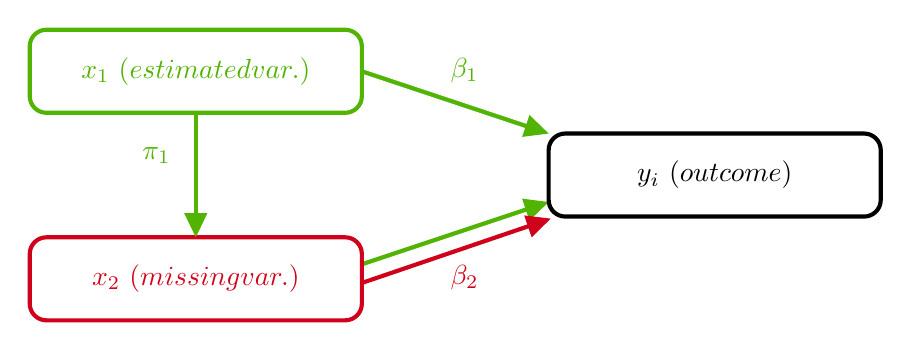
\begin{tikzpicture}[x=0.75pt,y=0.75pt,yscale=-1,xscale=1]
%uncomment if require: \path (0,361); %set diagram left start at 0, and has height of 361

%Straight Lines [id:da880895933850384] 
\draw [color={rgb, 255:red, 81; green, 179; blue, 2 }  ,draw opacity=1 ][line width=1.5]    (260,213) -- (346.21,184.26) ;
\draw [shift={(350,183)}, rotate = 161.57] [fill={rgb, 255:red, 81; green, 179; blue, 2 }  ,fill opacity=1 ][line width=0.08]  [draw opacity=0] (11.61,-5.58) -- (0,0) -- (11.61,5.58) -- cycle    ;
%Straight Lines [id:da6515543213351532] 
\draw [color={rgb, 255:red, 81; green, 179; blue, 2 }  ,draw opacity=1 ][line width=1.5]    (260,120) -- (346.21,148.74) ;
\draw [shift={(350,150)}, rotate = 198.43] [fill={rgb, 255:red, 81; green, 179; blue, 2 }  ,fill opacity=1 ][line width=0.08]  [draw opacity=0] (11.61,-5.58) -- (0,0) -- (11.61,5.58) -- cycle    ;
%Rounded Rect [id:dp051749207695209076] 
\draw  [line width=1.5]  (350,158) .. controls (350,153.58) and (353.58,150) .. (358,150) -- (502,150) .. controls (506.42,150) and (510,153.58) .. (510,158) -- (510,182) .. controls (510,186.42) and (506.42,190) .. (502,190) -- (358,190) .. controls (353.58,190) and (350,186.42) .. (350,182) -- cycle ;

%Rounded Rect [id:dp44940730713291466] 
\draw  [color={rgb, 255:red, 208; green, 2; blue, 27 }  ,draw opacity=1 ][line width=1.5]  (100,208) .. controls (100,203.58) and (103.58,200) .. (108,200) -- (252,200) .. controls (256.42,200) and (260,203.58) .. (260,208) -- (260,232) .. controls (260,236.42) and (256.42,240) .. (252,240) -- (108,240) .. controls (103.58,240) and (100,236.42) .. (100,232) -- cycle ;

%Rounded Rect [id:dp4060212389610093] 
\draw  [color={rgb, 255:red, 81; green, 179; blue, 2 }  ,draw opacity=1 ][line width=1.5]  (100,108) .. controls (100,103.58) and (103.58,100) .. (108,100) -- (252,100) .. controls (256.42,100) and (260,103.58) .. (260,108) -- (260,132) .. controls (260,136.42) and (256.42,140) .. (252,140) -- (108,140) .. controls (103.58,140) and (100,136.42) .. (100,132) -- cycle ;

%Straight Lines [id:da4471649391722271] 
\draw [color={rgb, 255:red, 81; green, 179; blue, 2 }  ,draw opacity=1 ][line width=1.5]    (180,140) -- (180,196) ;
\draw [shift={(180,200)}, rotate = 270] [fill={rgb, 255:red, 81; green, 179; blue, 2 }  ,fill opacity=1 ][line width=0.08]  [draw opacity=0] (11.61,-5.58) -- (0,0) -- (11.61,5.58) -- cycle    ;
%Straight Lines [id:da6210365408387567] 
\draw [color={rgb, 255:red, 208; green, 2; blue, 27 }  ,draw opacity=1 ][line width=1.5]    (260,222) -- (347.21,192.29) ;
\draw [shift={(351,191)}, rotate = 161.19] [fill={rgb, 255:red, 208; green, 2; blue, 27 }  ,fill opacity=1 ][line width=0.08]  [draw opacity=0] (11.61,-5.58) -- (0,0) -- (11.61,5.58) -- cycle    ;

% Text Node
\draw (430,170) node    {$y_{i} \ \text{(outcome)}$};
% Text Node
\draw (180,120) node    {$\textcolor[rgb]{0.32,0.7,0.01}{x_{1} \ \text{(estimated var.)}}$};
% Text Node
\draw (180,220) node    {$\textcolor[rgb]{0.82,0.01,0.11}{x_{2} \ \text{(missing var.)}}$};
% Text Node
\draw (309.5,119.5) node  [color={rgb, 255:red, 81; green, 179; blue, 2 }  ,opacity=1 ]  {$\beta _{1}$};
% Text Node
\draw (309.5,219.5) node  [color={rgb, 255:red, 208; green, 2; blue, 27 }  ,opacity=1 ]  {$\beta _{2}$};
% Text Node
\draw (161,160.5) node  [color={rgb, 255:red, 81; green, 179; blue, 2 }  ,opacity=1 ]  {$\pi _{1}$};


\end{tikzpicture}